\chapter{Appendix}
\section{Feature Map Normalization}\label{appendix:new_feature}
\begin{proof}
\begin{align*}
    \|
    \phi^{new}(x)\|_{\mathcal{H}}^{2} &= \|\frac{\phi(x)}{\|\phi(x)\|_{\mathcal{H}}}
    \|_{\mathcal{H}}^{2}
    \\
    &=
    \|
    \frac{\phi(x)}
    {\sqrt{k(x,x)}}
    \|_{\mathcal{H}}^{2}
    \\
    &=
    \langle
    \frac{\phi(x)}
    {\sqrt{k(x,x)}}
    ,
    \frac{\phi(x)}
    {\sqrt{k(x,x)}}
    \rangle_{\mathcal{H}}
    \\
    &=
    \frac{1}{\sqrt{k(x,x)^{2}}}
    \langle
    \phi(x)
    ,
    \phi(x)
    \rangle_{\mathcal{H}}
    \\
    &=1
\end{align*}
\end{proof}

\section{Cross validation}\label{appendix:cross_validation}



\section{Quantile regressor extensive comparison}\label{appendix:quantile_regressor_extensive_comparison}
\subsection{Boston housing dataset}
The Boston housing dataset \href{https://www.kaggle.com/datasets/altavish/boston-housing-dataset}{https://www.kaggle.com/datasets/altavish/boston-housing-dataset} contains information about various attributes for suburbs in Boston.
There are 13 indipendent variables:
\begin{itemize}
\item CRIM per capita crime rate by town
\item ZN proportion of residential land zoned for lots over 25,000 sq.ft.
\item INDUS proportion of non-retail business acres per town.
\item CHAS Charles River dummy variable (1 if tract bounds river; 0 otherwise)
\item NOX nitric oxides concentration (parts per 10 million)
\item RM average number of rooms per dwelling
\item AGE proportion of owner-occupied units built prior to 1940
\item DIS weighted distances to five Boston employment centres
\item RAD index of accessibility to radial highways
\item TAX full-value property-tax rate per 10,000
\item PTRATIO pupil-teacher ratio by town
\item B $1000(Bk - 0.63)^2$ where Bk is the proportion of afroamericans by town
\item LSTAT lower status of the population
\end{itemize}
The dependent variable is MEDV, that is the median value of owner occupied homes in \$1000's

\begin{table}
\caption{Pinball loss Boston housing data}
\begin{tabular}{lllll}
\toprule
    & Linear qr & Gbm qr & Quantile forest & Kernel qr \\
\midrule
0 & 13.785678 & 11.418540 & 10.587686 & 10.297572 \\
\bottomrule
\end{tabular}
\end{table}

\begin{table}
    \caption{Pinball loss quantile-wise Boston data}
\begin{tabular}{lllll}
\toprule
    & Linear qr & Gbm qr & Quantile forest & Kernel qr \\
\midrule
0.100000 & 0.729749 & 0.771714 & 0.588441 & 0.578898 \\
0.200000 & 1.122582 & 1.033442 & 0.932824 & 0.869145 \\
0.300000 & 1.479486 & 1.170642 & 1.153765 & 1.142783 \\
0.400000 & 1.712577 & 1.436263 & 1.352667 & 1.331955 \\
0.500000 & 1.911385 & 1.344361 & 1.408333 & 1.396300 \\
0.600000 & 1.989514 & 1.448885 & 1.464902 & 1.431705 \\
0.700000 & 1.938362 & 1.508741 & 1.427912 & 1.382772 \\
0.800000 & 1.658058 & 1.497901 & 1.275059 & 1.245288 \\
0.900000 & 1.243965 & 1.206591 & 0.983784 & 0.918725 \\
\bottomrule
\end{tabular}
\end{table}
        
\begin{table}
\caption{MAE Boston data}    
\begin{tabular}{lllll}
\toprule
    & Linear qr & Gbm qr & Quantile forest & Kernel qr \\
\midrule
0 & 3.826326 & 2.845989 & 2.965490 & 2.810494 \\
\bottomrule
\end{tabular}

\end{table}

\subsection{Abalone dataset}
The abalone data \href{https://archive.ics.uci.edu/dataset/1/abalone}{https://archive.ics.uci.edu/dataset/1/abalone} consist of measurements of abalone molluscs, the goal is predicting their age by building a model for estimating its number of rings; age is the number of rings plus 1.5
The data has 8 attributes:
\begin{itemize}
    \item Sex Categorical variable either male, female or infant
    \item Length
    \item Diameter
    \item Height
    \item Whole height
    \item Shucked height
    \item Viscera weight
    \item Shell weight
\end{itemize}

\begin{table}
    \caption{Pinball loss Abalone data}
\begin{tabular}{lllll}
    \toprule
     & Linear qr & Gbm qr & Quantile forest & Kernel qr \\
    \midrule
    0 & 5.613975 & 5.531938 & 5.212990 & 5.252491 \\
    \bottomrule
    \end{tabular}
\end{table}
    
\begin{table}
    \caption{Pinball loss quantile-wise Abalone data}
    \begin{tabular}{lllll}
    \toprule
     & Linear qr & Gbm qr & Quantile forest & Kernel qr \\
    \midrule
    0.100000 & 0.277903 & 0.290531 & 0.274079 & 0.269287 \\
    0.200000 & 0.469361 & 0.488079 & 0.453110 & 0.457286 \\
    0.300000 & 0.621961 & 0.625633 & 0.580766 & 0.596791 \\
    0.400000 & 0.729757 & 0.715875 & 0.689904 & 0.691310 \\
    0.500000 & 0.794695 & 0.766185 & 0.735945 & 0.740834 \\
    0.600000 & 0.810691 & 0.785769 & 0.744928 & 0.746636 \\
    0.700000 & 0.769587 & 0.730318 & 0.700287 & 0.710392 \\
    0.800000 & 0.667776 & 0.656913 & 0.609378 & 0.608334 \\
    0.900000 & 0.472244 & 0.472635 & 0.424593 & 0.431621 \\
    \bottomrule
    \end{tabular}
\end{table}
    
\begin{table}
    \caption{MAE Abalone data}
    \begin{tabular}{lllll}
    \toprule
     & Linear qr & Gbm qr & Quantile forest & Kernel qr \\
    \midrule
    0 & 1.627627 & 1.574179 & 1.499522 & 1.498583 \\
    \bottomrule
    \end{tabular}
\end{table} 

\subsection{Vehicle dataset}
This data contains info about used cars \href{https://www.kaggle.com/datasets/nehalbirla/vehicle-dataset-from-cardekho}{https://www.kaggle.com/datasets/nehalbirla/vehicle-dataset-from-cardekho}, the predictors are:
\begin{itemize}
    \item Year
    \item Present\_price ex showroom price
    \item Kms Driven
    \item Fuel type
    \item Seller type
    \item Transmission
    \item Owner number of previous owners
\end{itemize}
The dependent variable is the selling price.

\begin{table}
\caption{Pinball loss Vehicle data}
\begin{tabular}{lllll}
    \toprule
     & Linear qr & Gbm qr & Quantile forest & Kernel qr \\
    \midrule
    0 & 4.054449 & 2.289554 & 2.844410 & 2.204343 \\
    \bottomrule
    \end{tabular}
\end{table}

\begin{table}
    \caption{Pinball loss quantile-wise Vehicle data}
    \begin{tabular}{lllll}
    \toprule
     & Linear qr & Gbm qr & Quantile forest & Kernel qr \\
    \midrule
    0.100000 & 0.254649 & 0.139849 & 0.170489 & 0.182490 \\
    0.200000 & 0.403772 & 0.236339 & 0.285875 & 0.223165 \\
    0.300000 & 0.548820 & 0.244086 & 0.357375 & 0.242963 \\
    0.400000 & 0.576918 & 0.263169 & 0.389305 & 0.262835 \\
    0.500000 & 0.554367 & 0.306123 & 0.410738 & 0.295878 \\
    0.600000 & 0.563046 & 0.335363 & 0.398125 & 0.306062 \\
    0.700000 & 0.516019 & 0.287490 & 0.326572 & 0.283716 \\
    0.800000 & 0.407742 & 0.261882 & 0.313698 & 0.235793 \\
    0.900000 & 0.229115 & 0.215253 & 0.192233 & 0.171440 \\
    \bottomrule
    \end{tabular}
\end{table}

\begin{table}
    \caption{MAE Vehicle data}
    \begin{tabular}{lllll}
    \toprule
     & Linear qr & Gbm qr & Quantile forest & Kernel qr \\
    \midrule
    0 & 1.117714 & 0.606971 & 0.752197 & 0.594292 \\
    \bottomrule
    \end{tabular}
\end{table}
    

\section{Cross validation}
Cross validation directly estimates the expected test error
\begin{equation}
    Err=\mathbb{E}\left[L(Y,\hat{f}(X))\right]=\mathbb{E}\left[Err_{\tau}\right]
\end{equation}
$Err_{\tau}$ is the prediction error over an independent test sample
\begin{equation}
    \mathbb{E}_{\tau}=\mathbb{E}\left[L(Y,\hat{f}(X))| \tau \right]
\end{equation}
That is $Err$ is the average over everything that is random: X,Y and the training set $\tau$ used to generate $\hat{f}$. Hence, our interest lies in estimating the $Err$ quantity in order to guide model selection.
\subsection{K-fold cross validation}
K-fold cross validation splits the data into K roughly equal sized parts, then K models are trained. For k from 1 to K we train the kth model on the whole data except the kth partition. Next,  the prediction error of the kth fitted model when predicting the kth partition is computed. Finally averaging all the k prediction erros we obtain an estimate for its true value. We select the model which performs best in terms of expected prediction error.
\\
Usually, K is set equal to 5 or 10. Leave-one-out cross validation is the case when K is set equal to the size of the data.
% REMEMBER: Parameters allow the model to learn the rules from the data while hyperparameters control how the model is training. Parameters learn their own values from data. In contrast, hyperparameters do not learn their values from data. We need to manually specify them before training the model
\subsection{Gridsearch}
Model performance depends higly on the choice of hyperparameters. Notice, there is no way to get to know them in advance, therefore, all we can do is trying a lot of combinations until we fit a good enough set of hyperparameters. Essentially, gridsearch carries out hyperparameter tuning by performing a search over a predefined hyperparemeters grid. During its search, it tries all possible combination and evaluates the different models %(different hyperparameters define different models)
using cross validation. For example, supposing the grid contains 100 possible candidates and we are doing 5-fold cross-validation then we will be doing 500 iterations.
Therefore, we get an estimate of prediction error for each considered model and this guides us in hyperparameters(model) selection.

\subsection{Randomized search}
Randomizedsearch controls the number of step by choosing smartly the hyperparameter to try in each iterations.
Let us say there are 100 candidates and we set the number of iterations to 20 then the search will stop after the 20th iteration and return the best set among the hyperparameters observed.
The advantage is that it is much quicker than gridsearch, but on the other hand its performance is worse than gridsearch.

\subsection{Halving gridsearch}
Gridsearch has been the to go choice for hyperparameter tuning for the past years. However, such method is brute forcing all possible combinations, hence it is highly computationally intensive, especially when it comes to large datasets.
\\
The scikit-learn team addresses this disadvantage of gridsearch by introducing the halving gridsearch method \cite{scikithalvinggridsearch} (2020). Such technique has proved itself to greatly speed up hyperparameter tuning.
The ground concept underlying this method is successive halving. During the first iteration of halving gridsearch, all candidates are trained on a small subset of the training set. Next, we keep only the candidates which performed best and compare  them again on a bigger subset of the training set. As the iterations pass, the surviving candidates will be given more and more training samples until when we are left with only the best set of hyperparameters.

\subsection{Cross validation for time series data}
When data points are dependent on preceding values we cannot use standard K-fold cross validation. The rationale is that k-fold will randomize the order of the data, thus i might happen to use future data to predict the past; we want to avoid such behaviour in a time series setting. What we to have to keep in mind is that we must test our models during selection in the same way we will run them on the test dataset. Hence, for time series crossvalidation we have the TimeSeriesSplit procedure, see figure \ref{fig:crossvalidationtimeseries} for a visualisation.
\begin{figure}
    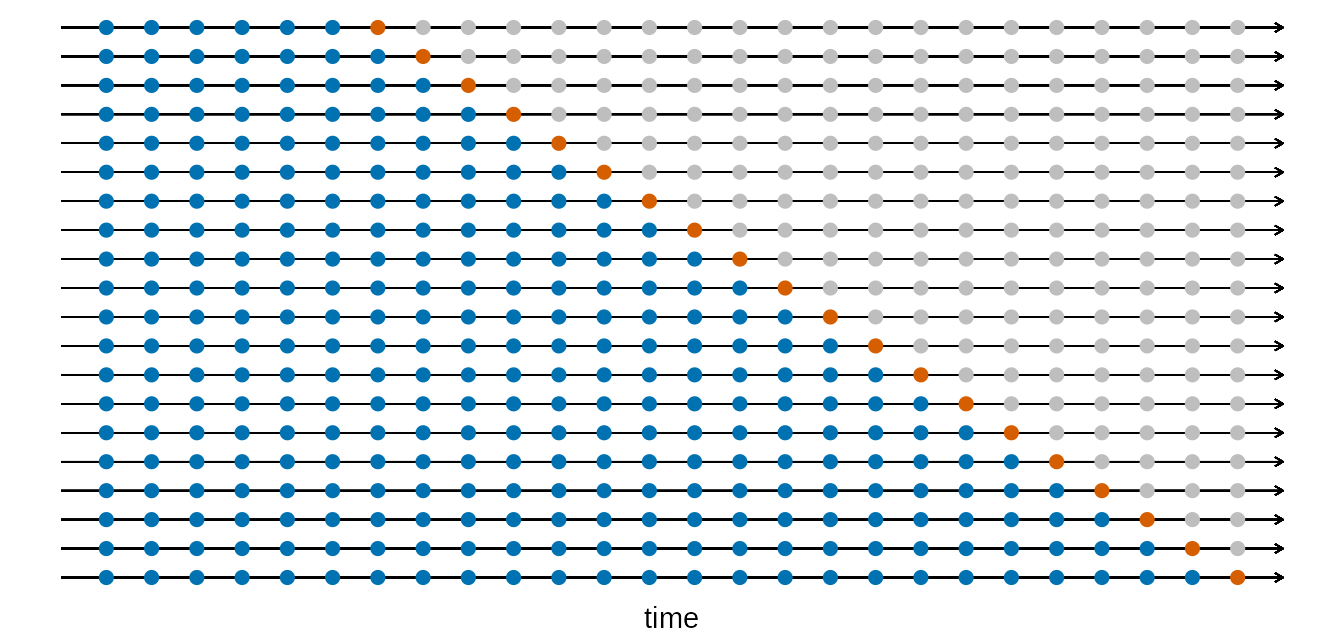
\includegraphics[width=\textwidth]{images/crossvalidationtimeseries.png}
    \caption{K-fold cross validation for timeseries data}
    \label{fig:crossvalidationtimeseries}
\end{figure}


\section{Kernel methods best practices}
Following, are reported a couple of considerations important to keep in mind when working with kernel methods.
\subsection{Data scaling}
\subsection{Data compression}
Nystrom, Cholesky

\newpage
\section{Src code}\label{src_code}
The whole code for the project is hosted on
\url{https://github.com/luca-pernigo/ThesisKernelMethods}\label{github_repo}.
\\
\begin{itemize}
    \item query: folder containing Scopus data and scripts to generate bibliometric survey plots in section \ref{literature_review}
    \item kqr.py: file implementing our custom kernel quantile regression
\end{itemize}
